\chapter{Architecture and Design}
This chapter describes a little bit about the overview of the plugin, the programming language that was used, how the plugin is deployed, what it needs in order to be executed successfully etc. It also describes why that specific programming language and the libraries were chosen and the main reasons sitting behind those decisions.\\
\hyperref[sec:ThePlugin]{The Plugin} section of this chapter describes the plugin in a more-depth manner, some of the libraries that were used, how it is bundled together and the components that are crucial to the plugin.
\section{Overview}
The plugin is developed and built using the \href{https://www.java.com/en/}{Java} programming language (Java Platform SE 8), which is fully compliant with the JOSM development environment (JOSM also supports higher Java versions). The plugin is developed as a "separate" component from JOSM, which can be manually added/installed to an existing JOSM application environment.\\
\newline
The plugin is ultimately deployed as a single \textit{.jar} file, which contains all the necessary components, dependencies and libraries that the plugin needs in order to execute successfully. This jar file however, does not serve its purpose if executed solely, it requires a JOSM application environment and must be executed from it in order for it to serve its purpose. It is a relatively heavy .jar file because of the XML components that it has bundled within, which boil down to a Java Model of the whole NeTEx XML schema containing all its components, their necessary interrelations and methods.

\section{Design Decision - Programming Language}
This plugin was built using the Java programming language, version 8.\\
\newline
\href{https://www.java.com/en/}{Java} is a powerful general-purpose programming language. It is used to develop desktop and mobile applications, big data processing, embedded systems, and so on. According to Oracle, the company that owns Java, Java runs on 3 billion devices worldwide, which makes Java one of the most popular programming languages. \cite{WhatIsJava}\\
\newline
The reason why this plugin was chosen to be built and developed using Java is because of JOSM, it runs on Java, so everything under it must run on Java too, including the plugins. All of the JOSM plugins are developed inside the JOSM environment as separate .jar files and must use JOSM native Java methods in order to be executed and incorporated within JOSM.\\
It is also an Object-Oriented programming language, which runs under ANY operating system (because of it's compiler) and uses inheritance and abstract methods (Object Oriented programming principles), which turned out to be very useful and neat for the nature of this plugin.\\
\newline
Here's a snippet of Java code \& syntax example of a Java Program that computes the quotient and the remainder of a division: \cite{JavaExampleQuadraticEquation}
\begin{minted}{java}
public class QuotientRemainder {
	
	public static void main(String[] args) {
		
		int dividend = 25, divisor = 4;
		
		int quotient = dividend / divisor;
		int remainder = dividend % divisor;
		
		System.out.println("Quotient = " + quotient);
		System.out.println("Remainder = " + remainder);
	}
}
\end{minted}
And the result from running the program would be:
\begin{minted}{bash}
Quotient = 6
Remainder = 1
\end{minted}
\newpage
\section{The Plugin}
\label{sec:ThePlugin}
\href{https://wiki.openstreetmap.org/wiki/JOSM/Plugins}{JOSM Plugins} extend or modify the feature set of the JOSM editor. \cite{JOSMPlugins}\\
That is the main purpose of these plugins. They are created by the JOSM community of developers and they tend to improve JOSM usability by adding extra or "missing" functionality, or in the most cases, by adding a completely new feature that interacts with JOSM components but serves an exclusive purpose.\\
There exist plugins for improving the look \& feel of drawing different shapes of objects within JOSM, for converting OSM data into various formats (which is our case), for exporting OSM data into formats such as PDF or GPX, for showing additional important information to some users etc.\\
\newline
This plugin is a single executable .jar file which runs under JOSM and is executed within it. It is developed by following the official JOSM development guidelines and OSM rules. The plugin, if installed on the JOSM environment, is first executed using a JOSM native library which takes care of plugin initialization, execution and error handling. After loaded into JOSM, depending on the nature of the plugin, it can interact with any component within JOSM, in this case, the plugin is a single option on the toolbar menu that simply takes the currently loaded map data in the main map layer and converts it into the NeTEx format. \\
\begin{figure}[H]
	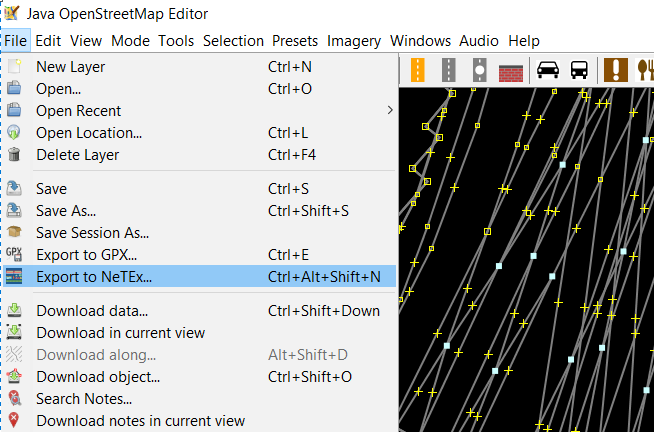
\includegraphics[width=\linewidth]{./Images/ArchitectureDesign/netex_converter_toolbar.png}
	\caption{The location of the NeTEx Converter plugin within the JOSM toolbar}
\end{figure}
After the conversion is completed, any log information (warning, error) will be displayed within the JOSM map layer by highlighting the intended object, may that be a node, a way or even a relation.
\begin{figure}[H]
	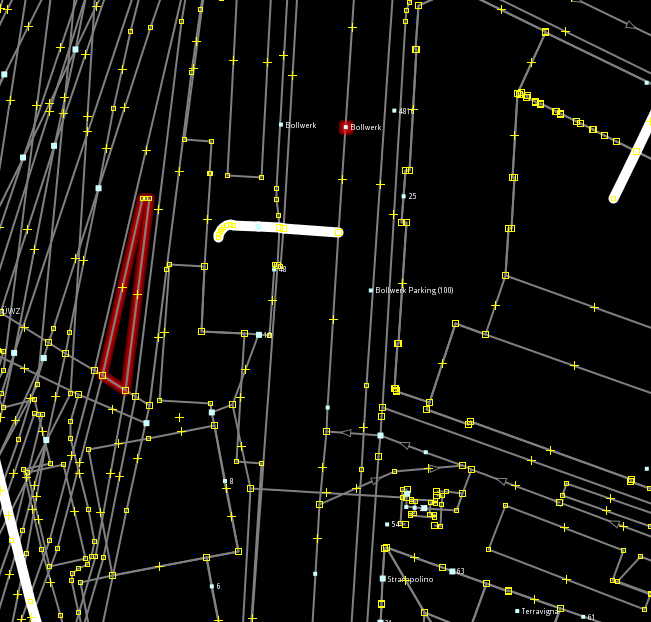
\includegraphics[width=\linewidth]{./Images/ArchitectureDesign/highlight_example.png}
	\caption{An example of the plugin highlighting objects that need attention after a conversion (Location - Bern, Switzerland)}
\end{figure}
After identifying the highlighted objects, if we click on them, on the tags of the object, there will be a tag with a message corresponding to the action/s that need/s to be taken in order to improve that object so that the future NeTEx conversions are refined.\\
All of the tags generated by the plugin that need attention have a suffix of "\textit{ - (NeTeX Converter)}".


